\chapter{Analiza problemu}
\thispagestyle{chapterBeginStyle}
\label{rozdzial1}
Rozdział ten skupia się na analizie dotychczasowych podejść do problemu generowania liczb losowych, jak również zarysowaniu koncepcji naszego podejścia do problemu. Dodatkowo zostanią tu również zaprezentowane podstawowe trudności wynikające z wybranej metody, wraz z ich konsekwencjami dla implementacji generatora.

\section{Czy można stworzyć prawdziwy generator liczb losowych?}
Zanim przejdziemy do stworzenia konceptu warto zadać sobie pytanie, czy w ogóle generator spełniający założenia pracy może istnieć? Naszą wątpliwość możemy sprowadzić do problemu, czy świat jest deterministyczny, czy też nie. Naturalnie w deterministycznym świecie każda akcja bezpośrednio wynika ze stanu początkowego. Znając go, w naszym przypadku stan całego wszechświata, moglibyśmy zasymulować wszystkie kolejne stany, a co za tym idzie również wyniki naszego systemu. Przy takich założeniach każdy generator byłby jedynie generatorem liczb pseudolosowych, z bardziej lub mniej złożoną zasadą działania. Jeśli natomiast nasz świat nie jest deterministyczny, możemy użyć tej niepewności do generowania prawdziwie losowego ciągu.
\subsection{Debata nad wolną wolą}
Jedynym z pierwszych miejsc, w których możemy znaleźć niepewność we wszechświecie jesteśmy my sami, a bardziej precyzyjnie - ludzka wolna wola, czyli zdolność do podjęcia w tych samych okolicznościach i z tymi samymi wspomnieniami, przekonaniami, myślami itp. dwóch różnych decyzji. Założenie wolnej woli jest dla ludzi bardzo intuicyjne; każdy z nas przecież czuje się zdolnym do podejmowania różnych decyzji. Jedną z nich był wybór przeczytania niniejszej pracy nad wszystkimi innymi możliwościami spędzenia tego czasu. Jednak oprócz naszego poczucia wolnej woli trudno znaleźć naukowe przesłanki świadczące o niej. Już od starożytności ludzkość zadaje sobie pytanie o to czy ma wpływ na swój własny los. Dzieła takie jak \emph{Król Edyp} \cite{Edyp} autorstwa Sofoklesa przedstawiają wizję, w której wszytko jest z góry zdeterminowane, a ucieczka przed przeznaczeniem (determinizmem wszechświata) jest niemożliwa. Jednym z największych krytyków idei wolnej woli był francuski filozof z epoki oświecenia Paul d'Holbach, który w swoim dziele \emph{Systemy przyrody} \cite{baron} stwierdził, że ludzki mózg poddaje się prawom fizyki jak każdy inny fizyczny obiekt, więc tak jak inne obiekty poddaje się determinizmowi, a nasze decyzje możemy sprowadzić do wypadkowej naszych przekonań, pragnień oraz naszego usposobienia. Uznał zatem, że istnienie wolnej woli stoi w sprzeczności z prawami natury.
\subsection{Fizyka kwantowa jako źródło entropii}
Od czasów dzieł Paula d'Holbacha dokonaliśmy sporego rozwoju naszego zrozumienia fizyki. Pojawiła się nieznana w jego czasach mechanika kwantowa. Obecnie konsensus naukowy mówi, że pozycja cząstek elementarnych nie jest jednym miejscem, a raczej funkcją prawdopodobieństwa \cite{Quantum}, gdzie może się ona znajdować. Zakładając, iż rzeczywiście tak jest można by wykorzystać to źródło niepewności do generowania liczb losowych. Jednak fizyka wciąż się rozwija i istnieje spore ryzyko, że tak naprawdę ta losowość jest jedynie pewnym uproszczeniem bardziej skomplikowanego modelu, którego jeszcze nie rozumiemy. Dlatego też pytanie na temat determinizmu świata nadal pozostaje otwarte i najprawdopodobniej nigdy nie poznamy na nie jednoznacznej odpowiedzi.

\section{Dostępne rozwiązania problemu generowania liczb losowych}
Problem generowania liczb losowych jest prawie tak stary jak same komputery. Pierwsze rozwiązania tego zagadnienia przypisujemy Johnowi von Neumannowi, który w 1949 roku opisał swój pomysł generowania liczb o trudnym do przewidzenia wzorcu (\emph{metoda środkowego kwadratu} \cite{msm}). Od tego czasu powstały dwa różne podejścia do tego problemu: generatory liczb pseudolosowych oraz ''prawdziwe'' generatory liczb losowych.
\subsection{Generatory liczb pseudolosowych}
Są to metody algebraiczne polegające na generowaniu ciągu liczb opisanego pewnym wzorem. Jest on na tyle skomplikowany, aby wydawało się, iż elementy tego ciągu nie mają żadnego związku między sobą. Użycie następującego rozwiązania ma wiele zalet:
\begin{description}
\item[uniwersalność:] z uwagi na to, że rozwiązanie opiera się jedynie na operacjach arytmetycznych może być ono zastosowane na każdej programowalnej maszynie liczącej, uwzględniając bardzo prymitywne mikrokontrolery. Umożliwia to również uruchamianie takiego programu w środowisku chronionym, czyli takim w którym program nie powinien mieć dostępu do informacji z zewnątrz. Cechy te sprawiają, iż praktycznie każdy język programowania ma wbudowany jakiś generator liczb pseudolosowych czyniąc je łatwym wyborem dla programistów.
\item[wysoka wydajność:] zdecydowana większość rozwiązań tego typu charakteryzuje się bardzo szybką metodą generowania kolejnych elementów ciągu. Wygenerowanie ciągu długości $n$ zajmuje asymptotycznie $O(n)$ czasu i $O(1)$ pamięci. Kolejnym aspektem jest to, że przy tego typu generatorach ogranicza nas jedynie wydajność procesora. Dlatego też możemy łatwo wykorzystać cały potencjał naszego sprzętu przy rozwiązywaniu problemów wymagających dużej liczby liczb losowych. Dobrym przykładem są tutaj algorytmy wykorzystujące metodę Monte Carlo, wymagają one dużej ilości próbek, stąd też w większości decydują się na pseudolosowość.
\item[jednostajność:] jako że tego typu generatory są w pełni deterministyczne, możemy często udowodnić iż mają one oczekiwany jednostajny rozkład. Jest to duża zaleta w zastosowaniu tego podejścia w wyżej wspominanych algorytmach wykorzystujących metodę Monte Carlo. Pozwala ona uniknąć nieprawidłowości wynikających z nadreprezentacji pewnych liczb.
\end{description}
Pomimo tylu zalet rozwiązanie to nie jest pozbawione kilku istotnych wad:
\begin{description}
\item[problem stanu początkowego (\tetxit{seedu}):] ciągi pseudolosowe są deterministyczne, a więc dla tych samych warunków początkowych wygenerowane ciągi będą identyczne. Stąd pojawia się potrzeba wygenerowania stanu początkowego wykorzystując inną metodę generowana liczb losowych. Najczęściej w tym celu stosuje się czas uruchomienia, co może być jednak zgubne w przypadku programów uruchamianych cyklicznie. Zastosowanie generatorów tego typu do rozpoczęcia prawidłowej pracy wymaga odrobiny entropii z zewnątrz, na szczęście nie musi ona spełniać tak rygorystycznych wymagań jak nasz generator. Osłabia to jednak nieco uniwersalność tego rozwiązania.
\item[brak niezależności:] jest to największy problem tego podejścia. Jako iż nasz generator wykonuje jedynie szereg deterministycznych obliczeń, znając warunki początkowe i użyty algorytm, możemy bez problemu wygenerować identyczny ciąg. Bardziej wyrafinowane współczesne generatory tego typu posiadają rozbudowany stan wewnętrzny, a więc wyznaczenie kolejnej liczby na podstanie jedynie kilku poprzednich jest niemożliwe. Jednak przy pozyskaniu odpowiedniej liczy próbek z generatora możliwe jest wyznaczenie jego stanu wewnętrznego, a co za tym idzie, również odtworzenie identycznego ciągu jaki produkuje nasz generator. Stąd też w zastosowaniach kryptograficznych nie zalecane jest używanie generatorów liczb pseudolosowych.
\item[zapętlanie się:] problem ten wynika z prostej obserwacji, iż w komputerze generator może mieć jedynie skończoną liczbę stanów wewnętrznych oraz tego, iż stan wewnętrzny w pełni determinuje kolejne uzyskiwane wyniki. Tak więc dla każdego generatora i każdego stanu początkowego istnieje taka liczba $l$,  że $( \forall{k} \in \mathbb{N} ) X_{k} = X_{k+l} $. W bardziej zaawansowanych generatorach liczba $l$ jest bardzo wysoka, rzędu $2^{100}$, co niweluje ten problem.
\end{description}
\subsection{''Prawdziwe'' generatory liczb losowych}
Rozwiązania z tej kategorii opierają swoją losowość na informacjach pochodzących ze świata zewnętrznego. Ilość czynników jakie oddziałują na środowisko, w którym działa maszyna jest olbrzymia, stąd też istnieje niesamowita różnorodność podejść w tworzeniu tego typu generatorów. Jednymi z najpopularniejszych są: pomiar różnicy temperatury, wsłuchiwanie się w szum elektromagnetyczny lub, jeśli to możliwe, obserwowanie zachowania użytkownika systemu. Warto wymienić tutaj podstawową zaletę tej metody:
\begin{description}
\item[prawdziwa niezależność:] to podejście pozwala nam spełnić drugie z wymienionych wymagań dotyczących generatorów liczb losowych. Nawet jeśli świat byłby deterministyczny, to zjawisko jakim jest efekt motyla generuje dostatecznie dużo niepewności, żeby żaden komputer stworzony przez człowieka nie był w stanie przewidzieć rezultatów. Najlepszym z ''dowodów'' na to jest fakt, iż pomimo lat starań i dużego zapotrzebowania na długoterminowe prognozy meteorologiczne nikt nie umie przewidzieć pogody na okres dłuższy niż 2 tygodnie. Wyobraźmy sobie generator oparty na temperaturze powietrza. Na potrzeby jego analizy nieco uprośćmy obraz świata zewnętrznego. Powiedzmy, że na zmianę temperatury wpływa jakaś ogromna liczba $M$ binarnych zdarzeń takich jak to, czy motyl w parku lata czy nie. Stosując centralne twierdzenie graniczne wiemy, że rozkład prawdopodobieństwa temperatury w następnej chwili powinien być podobny do rozkładu normalnego, a co za tym idzie na odpowiednio małym wycinku czasu przypominać będzie jednowymiarowy ruch Browna. A więc na 50\% temperatura powinna się podnieść i na 50\% powinna się obniżyć.
\end{description}
Podejście to jest nie jest jednak pozbawione wad:
\begin{description}
\item[wolne generowanie liczb:] głównym problemem w tym podejściu jest fakt, że niezależnie od mocy obliczeniowej urządzenia możemy uzyskać tylko ograniczoną ilość próbek w ciągu sekundy. Pomimo założenia, iż parametry świata rzeczywistego mają charakter ciągły tzn. nasza temperatura płynnie zmienia się w czasie, to jednak komputery są maszynami skończonymi. Co za tym idzie nie są w stanie dokładnie odczytać parametru ze świata zewnętrznego, a jedynie jego zniekształcony cyfrowy obraz. Ma on tą cechę, iż rzutuje całe przedziały np. $[0, 1)$ na pojedynczą wartość 0.
\begin{figure}[!htp]
    \centering
    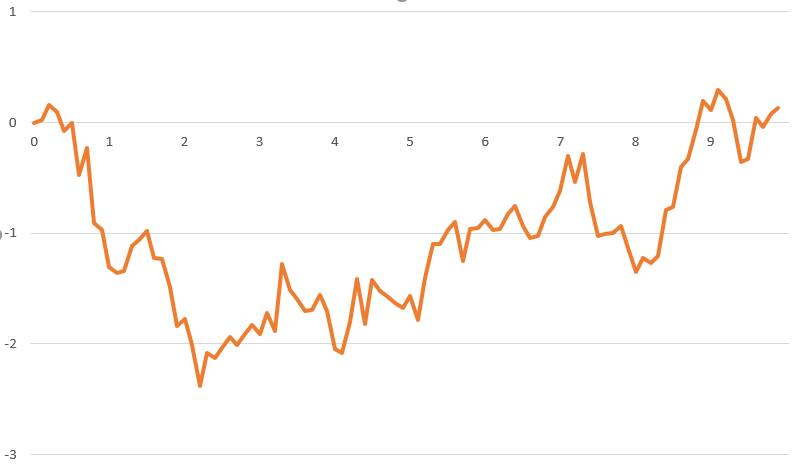
\includegraphics[width=10cm]{brown}
    \caption{Przykładowy jednowymiarowy proces Weinera (ruch Browna)}
    \label{fig:brown}
\end{figure}
Jak możemy zaobserwować na rysunku \ref{fig:brown} pomimo, iż wysokość wykresu ciągle się zmienia, to często wahania te pozostają w granicach przedziału precyzji. A więc wykonanie pomiaru w 6 i 7 sekundzie wyprodukuje identyczny rezultat. Stąd też wymagają czasu, aby temperatura zmieniała się na tyle, żeby nasz system był w stanie wykryć różnicę. Częstym problemem jest również sama ilość próbek, które urządzenie pomiarowe jest w stanie w ciągu sekundy wygenerować urządzenie pomiarowe.
\item[ryzyko manipulowania wynikami:] świat zewnętrzy jest niemożliwy do kontrolowania z punku widzenia twórcy sytemu. Istnieje więc ryzyko, iż osoba posiadająca dostatecznie dużo wiedzy na temat działania pewnego systemu tworzącego liczby losowe będzie w stanie manipulować warunkami środowiskowymi na tyle, żeby wygenerował oczekiwany przez nią rezultat. Możemy np. ciągle ogrzewać czujnik temperatury tak, żeby nigdy nie pokazał, iż temperatura spada lub wręcz sprawić, żeby przekroczył on zakres swoich odczytów.
\item[dostęp do świata zewnętrznego:] w celu pobrania informacji o jakimś parametrze ze świata zewnętrznego konieczny jest czujnik, który jest w stanie odczytać jego wartość. Co oczywiście, nie jest możliwe zmierzenie temperatury bez termometru. W celu generowania odpowiedniej liczby próbek potrzebny jest jednak odpowiedniej klasy sprzęt pomiarowy podnosząc tym samym koszty produkcji urządzenia, który takowy posiada. Stąd tego typu moduły nie są popularne, zwłaszcza w tanich urządzeniach. Pewnym obejściem problemu jest wykorzystanie użytkownika jako źródła entropii dla systemu. Jest to jednak rozwiązanie relatywnie wolne i może być zastosowane jedynie w systemach, w których występuje interakcja z użytkownikiem.
\item[niepewność jednostajności liczb losowych:] oderwanie się od matematycznych wzorów powoduje, iż nie możemy przeprowadzić dowodu poprawności działania takich generatorów. Sprawia to, że nie możemy być pewni parametrów rozkładu naszych zmiennych losowych. Zapewnienie jego jednostajności jest jedną z największych trudności w tym podejściu.
\end{description}

\section{Koncept generatora}
Generator spełniający oba wymagania sprecyzowane w celu tej pracy musi należeć do kategorii ''prawdziwych'' generatorów liczb losowych. Tak więc będzie on wykorzystywać informacje o świecie zewnętrznym celem generowania kolejnych liczb losowych.
\subsection{Źródło entropii}
W tym celu wykorzystamy opóźnienia w przesyłaniu pakietów przez sieć globalną. Jednym powodem ich powstawania na drodze naszego pakietu będzie obciążenie hosta docelowego. Jest on praktycznie zupełnie poza naszą kontrolą i wynika z liczby użytkowników chcących pobrać z niego informacje, a więc jest wypadkową tysięcy niezależnych od nas decyzji ludzkich jak i również zautomatyzowanych systemów. Pomiędzy naszym komputerem, a hostem docelowym występuje pewna liczba komputerów (routerów) odpowiedzialnych za przekierowywanie pakietów do celu. Każdy z tych routerów również generuje opóźnienia wynikające z ich obecnego obciążenia. Tak więc nawet jeśli jako jedyni chcemy sprawdzić ceny akcji firmy \emph{Apple}, to na czas uzyskania tych informacji ma również wpływ sąsiadka wyszukującą w Internecie filmiki z kotami. Ostatnim z źródeł opóźnień na drodze pakietu jest czas jego przetworzenia przez nasz komputer co więcej, że warunki środowiskowe takie jak temperatura powietrza, opady atmosferyczne czy nawet promieniowanie kosmiczne na trasie pakietu mają również pewien, choć bardzo niewielki wpływ na jego czas podróży.  
\subsection{Przekształcenie próbek na liczby losowe}
Posiadając już odpowiednio losowe źródło entropii, którym dla naszego przypadku będzie dodatnia liczba naturalna określająca czas podróży pakietu w pewnej jednostce czasu, należy je jeszcze odpowiednio przetworzyć, aby zapewnić oczekiwany jednostajny rozkład liczb losowych. W przypadku tej pracy, w tym celu ''obetniemy'' każdą próbkę do najmniej znaczących bitów, używając w tym celu operacji modulo. Część z bitów naszej próbki powinna mieć rozkład statystycznie nieróżniący się od rozkładu jednostajnego.

\section{Występowanie prawa Benforda w rozkładzie czasów dostępów}
\subsection{Definicja}
Rozkład zmiennej losowej $X$ spełnia prawo Benforda wtedy i tylko wtedy gdy $Lead(X)$ (funkcja zwracająca najbardziej znaczącą cyfrę) spełnia warunek \ref{eq:benford_def}:
\begin{equation}
    \label{eq:benford_def}
    P(\textrm{Lead}(X) = d) = \log_b(d+1)-\log_b(d) = \log_b\left(1+\frac{1}{d}\right)
\end{equation}
gdzie $b$ oznacza podstawę systemu liczbowego w którym zapisana jest dana liczba.
\subsection{Historia}
Pierwszym opublikowanym artykułem na temat tego fenomenu jest \emph{Note on the frequency of use of the different digits in natural numbers} (tłum. \emph{Uwaga na temat częstotliwości występowania różnych cyfr w liczbach naturalnych}) \cite{first_benford}. W nim właśnie Simon Newcomb podzielił się obserwacją, iż najbardziej znaczące cyfry (1-9) nie występują w jednakowej proporcji. Swojego odkrycia dokonał, gdy zauważył że pierwsze strony książki zawierającej wyliczone logarytmy są bardziej  zniszczone niż dalsze. Zaproponował on przedstawioną wyżej formułę opisującą to zjawisko. Kolejnym matematykiem zajmującym się tym problemem był Frank Benford. Na podstawie danych z kilkunastu dostępnych baz danych zauważył on, że około połowa z nich spełnia nazwane od jego nazwiska prawo Benfoda \cite{benford}. Formalizacji tego fenomenu dokonał amerykański matematyk Ted Hill \cite{hill}.
\subsection{Uogólnienie na dalsze cyfry}
Posiadając podaną wyżej definicję prawa Benforda możemy łatwo uogólnić ją na dalsze cyfry. Aby tego dokonać należy zmienić podstawę systemu z $b$ na $b^{k}$ (gdzie $k$ jest $k$-tą najbardziej znaczącą cyfrą). Teraz możemy obliczyć prawdopodobieństwo występowania każdej $k$ cyfrowej kombinacji na początku. Należy jednak pamiętać, że dopuszczalne kombinacje muszą być większe bądź równe $b^{k-1}$, gdyż w przeciwnym wypadku na pierwszej pozycji takiej kombinacji będzie występowało zero, a więc nie będzie to najbardziej znacząca cyfra. Z tych obserwacji możemy wyciągnąć formułę \ref{eq:benford_gen}.
\begin{equation}
\label{eq:benford_gen}
    \begin{split}
        & P(\textrm{Lead}_k(X) = d) = \\
     & = \log_b\left(1+\frac{1}{b^{k-2}+d}\right) + \log_b\left(1+\frac{1}{b^{k-2}+b+d}\right) + \dots + \log_b\left(1+\frac{1}{b^{k-1}-b+d}\right) = \\
     & =  \sum_{n=b^{k-2}}^{n=b^{k-1}-1}\log_b\left(1+\frac{1}{b n+d}\right)
    \end{split}
\end{equation}
Jak widzimy, obliczenie prawdopodobieństwa każdej kolejnej z cyfr jest wykładniczo bardziej złożone.
\subsection{Obserwacja}
Zgodnie z naszymi założeniami początkowymi moglibyśmy się spodziewać, że ze względu na ogromną ilość czynników mających wpływ na czas dostępu jego rozkład powinien dążyć do rozkładu normalnego ze względu na centralne twierdzenie graniczne. Problematycznym w tej tezie jest natomiast fakt, iż czas dostępu nie może być ujemny. Tak więc dla wartości oczekiwanej rozkładu $M$, prawdą jest, iż $P(X \in [-M, 0]) < P(X \in [2M, 3M])$. Być może jednak wartości tak oddalone od wartości oczekiwanej i tak są pomijalne w całym rozkładzie. 
\begin{figure}[!htp]
    \centering
    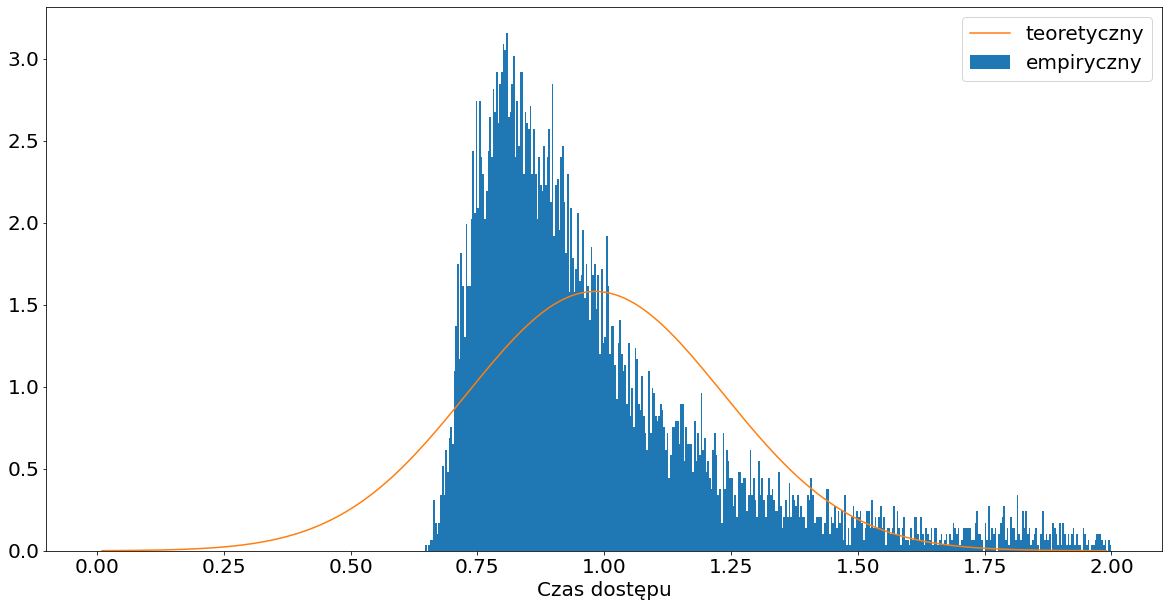
\includegraphics[width=15cm]{norm-ping-dist}
    \caption{Porównanie histogramu czasu dostępu do strony \url{https://www.spaceneedle.com/} z gęstością rozkładu noramlnego}
    \label{fig:bad_dist}
\end{figure}
Jak możemy zobaczyć na rysunku \ref{fig:bad_dist}, rozkład teoretyczny nie pokrywa się empirycznym. Musimy zatem zrewidować swoją tezę. Dokonujemy obserwacji, że $P(X \in [\frac{1}{2}m, m]) \approx P(X \in [m, 2m])$. Możemy zatem postawić hipotezę, iż mamy do czynienia z rozkładem logarytmicznym, precyzyjniej postawimy hipotezę o rozkładzie log normalnym.
\begin{figure}[!htp]
    \centering
    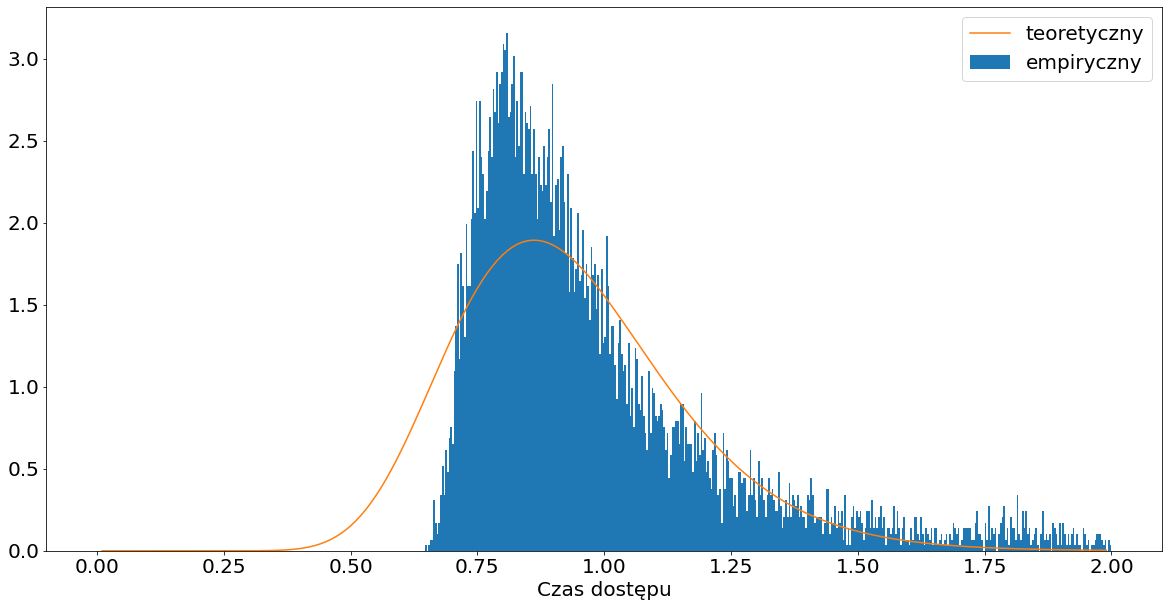
\includegraphics[width=15cm]{lognorm-ping-dist}
    \caption{Porównanie histogramu czasu dostępu do strony \url{https://www.spaceneedle.com/} z gęstością rozkładu log noramlnego}
    \label{fig:better_dist}
\end{figure}
Jak widzimy na wykresie \ref{fig:better_dist} rozkład log normalny lepiej pasuje do empirycznego histogramu. Możemy zatem sprawdzić, czy wygenerowane liczby spełniają prawo Benforda. Jako, iż mamy do czynienia z komputerami, będziemy pracować z systemem liczbowym o podstawie 2.
\begin{table}[H]
\begin{center}

\begin{tabular}{|l|r|}
\hline
Pozycja & \multicolumn{1}{l|}{Prawdopodobieństwo wystąpienia 1} \\\hline
1       & 1                                                    \\\hline
2       & 0.41503749927884376                                  \\\hline
3       & 0.4556794837761896                                   \\\hline
4       & 0.47755858383690225                                   \\\hline
5       & 0.48874172051300435                                   \\\hline
6       & 0.49436607559162077                                  \\\hline
7       & 0.49718243682965746                                 \\\hline
8       & 0.4985911432029018                                  \\\hline
9       & 0.4992955621971009                                   \\\hline
10      & 0.49982388981450276                                   \\\hline
\dots     & \dots                                                  \\\hline
20      & 0.4999996560346523                                   \\\hline
\dots     & \dots                                                  \\\hline
$\infty$& 0.5 \\\hline                                                
\end{tabular}
    
\end{center}
\caption{\label{tab:benford}Rozkład prawdopodobieństwa występowania 1 na pozycji licząc od najbardziej znaczącej}
\end{table}
W tablicy \ref{tab:benford} możemy znaleźć teoretyczne prawdopodobieństwa występowania 1 na $k$-tym najbardziej znaczącym miejscu.
Porównajmy zatem na rysunku \ref{fig:benford_in_real} uzyskane próbki z teoretycznymi prawdopodobieństwami występowania jedynki na $k$-tej najbardziej znaczącej pozycji.
\begin{figure}[!htp]
    \centering
    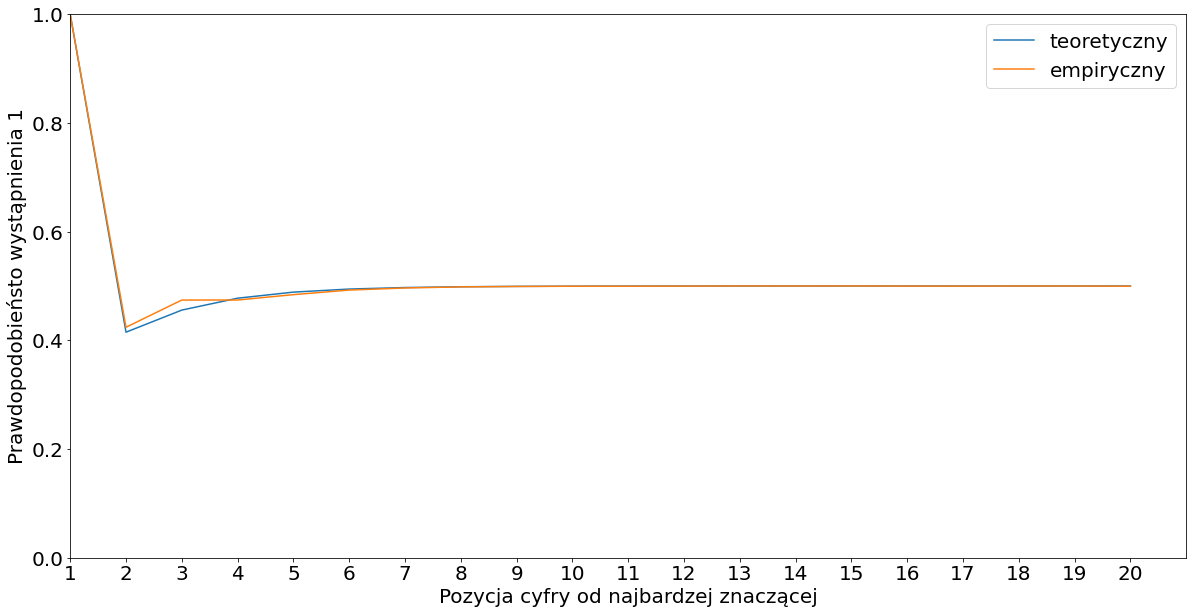
\includegraphics[width=15cm]{benford_comp}
    \caption{Porównanie teoretycznego prawdopodobieństwa występowania '1' na $k$-tej najbardziej znaczącej pozycji (linia niebieska), z empirycznym prawdopodobieństwem (linia pomarańczowa) }
    \label{fig:benford_in_real}
\end{figure}
\subsection{Konsekwencje}
Jak możemy dostrzec na wykresie \ref{fig:benford_in_real}, prawo Benforda dość dobrze opisuje zaobserwowane odchylenie od rozkładu jednostajnego.
Fakt ten rodzi problem przy próbie przekształcenia próbki na ciąg zmiennych losowych o binarnym rozkładzie $(P(X = 0) = \frac{1}{2} \land P(X = 1) = \frac{1}{2})$. Prosta konwersja liczby zmiennoprzecinkowej na ciąg bitów nie zapewni nam oczekiwanego rezkładu. Aby zatem zniwelować ten problem podczas generowania liczb o rozkładzie jednostajnym, wymagane będzie odrzucenie pewnej ilości początkowych bitów, których rozkład będzie najbardziej zaburzony prawem Benforda. Spowoduje to oczywiste obniżenie wydajności generatora w zależności od ilości odrzuconych bitów początkowych z każdej próbki. Konieczne pozostanie zatem balansowanie pomiędzy jednostajnością rozkładu a wydajnością generatora. 
\section{Maksymalna precyzja pomiaru}
\subsection{Jak komputery liczą czas?}
Współczesne komputery posiadają moduł \emph{RTC} (zegar czasu rzeczywistego), który służy jednak głównie do wyświetlania aktualnego czasu, przez co jego precyzja nie jest wystarczająca aby mierzyć czas wykonywania operacji na komputerze. Dlatego też wciąż wykorzystuje się przerwania na procesorze wykonywane co pewną stałą ilość cykli, podczas których następuje inkrementacja licznika czasu. Nie mogą być one jednak zbyt częste, żeby nie obciążać niepotrzebnie maszyny. Oczywiście implementacja tego rozwiązania różni się mocno pomiędzy komputerami, stąd ten sam program może lepiej lub gorzej mierzyć czas w zależności od sprzętu, na którym jest uruchomiony. Dla procesorów o częstotliwości kilku giga Hertzów ($10^9$ operacji na sekundę) precyzyjne odmierzanie upływu nanosekund ($10^{-9}$ części sekundy) zajęłoby większość taktów procesora. Stąd też na takich maszynach możemy spodziewać się jedynie precyzji rzędu mikrosekund ($10^{-6}$ części sekundy). 
\subsection{Wpływ precyzji pomiaru na wydajność}
Precyzja pomiaru w oczywisty sposób wpływa na ilość bitów jakie możemy uzyskać z jednej próbki. Jeśli przymniemy, że uzyskane czasy dostępu będą miały wartości od 16ms do 512ms, to przy precyzji rzędu mikrosekundy możemy uzyskać od 14 do 19 bitów informacji. Zakładając zatem wykorzystanie tylko jednego wątku do tego zadania możemy uzyskać do 875 bitów na sekundę, co jest niewielką wartością, zwłaszcza w porównaniu z generatorami liczb pseudolosowych, które generują kilka kilobajtów danych na sekundę.
\subsection{Konsekwencje}
Taka niewielka ilość bitów uzyskanych z jednej próbki w oczywisty sposób wymusza konieczność zebrania ich większej ilości w celu wygenerowania pojedynczej liczby losowej. Nawet przy  założeniach, że wszystkie bity w tej próbce będą miały oczekiwany przez nas rozkład, przy 16 bitach informacji z każdej, będziemy potrzebować ich aż cztery, aby wygenerować 64 bitową liczbę. Każda próbka generuje obciążenie sieci. Jej przepustowość jest ograniczonym zasobem na każdej maszynie, co jest poważnym problemem w tej metodzie generowania liczb losowych.
